\section{Coordinating Guest OS States}
\label{sec:graphene:namespaces}

%\fixmedp{RF: what are the few, powerful mechanisms?  Expect that there are many cases 
%with shared state; re-read this to see if it is clear how to generalize the approach}

%Recent library OS designs focus on single-process applications,
%which move a substantial portion of the OS APIs and state used by the application into the \libos{}.

%A key contribution of the \graphene{} 
%design is robust and flexible support for multi-process applications.
An application executes on \graphene{} 
with the abstraction that all of its processes are running on a single OS.
\graphene{} \libos{}es service system calls
from local \libos{} state whenever possible,
and state is coordinated across \picoprocs{} via RPC when necessary.
Within a sandbox, \graphene{} \picoprocs{} 
coordinate shared state used to implement multi-process
abstractions, such as process identifiers, thread groups, and 
System V IPC including message queues and semaphores, shared file system and file descriptor states (Table~\ref{tab:graphene:multiproc}).
Similar to previous designs~\cite{porter11drawbridge,baumann13bascule}, 
\graphene{} uses the host file system; 
the \libos{} implements file handles and translates between POSIX and the host ABI.
Identifying the best division of labor for a \libos{} file system is 
left for future work.

\begin{comment}
\begin{table}
\footnotesize
\centering
\begin{tabular}{|p{0.9in}|p{1.5in}|p{3.6in}|}
\hline
{\bf Ab\-strac\-tion} & {\bf Shared State} & {\bf Strategy} \\
\hline
Fork & 
\raggedright
PID namespace & Batch allocations of PIDs, children generally created using local state at parent.  \\
\hline
Signaling & PID to \picoproc{} map & Local signals call handler; remote signal delivery by RPC.  Cache mapping of PID to \picoproc{} ID. \\
\hline
\raggedright
Exit notification & 
\raggedright
Remote process status  & Exiting processes issue an RPC, or one synthesized if child becomes unavailable.  The {\tt wait} system call blocks until notification received by IPC helper. \\
\hline
{\tt /proc/[pid]} & Process metadata & Read over RPC.  \\
\hline
Message Queues & 
\raggedright
Key mapping, queue contents & Mappings managed by a leader, contents stored in various \picoprocs{}.  When possible, send messages asynchronously, and migrate queues to the consumer.\\
\hline
Semaphores & 
\raggedright
Key mapping, count. & Mappings managed by leader, migrate ownership to \picoproc{} most frequently acquiring the semaphore. \\
\hline
\raggedright
File System & 
\raggedright
File truncate sizes, FIFO files, domain sockets, symbolic links, file locks & No coordination, create special files in the host to represent symbolic links and file locks. \\
\hline
\raggedright
Shared File Descriptors & 
\raggedright
Seek pointers & Mappings managed by parent, migrate ownership to \picoproc{} most frequently accessing the file descriptors. \\
\hline
\end{tabular}
\caption[Multi-process abstractions implemented in sysname{}]
{Multi-process abstractions implemented in \graphene{}, coordinated state, and implementation strategies.}
\label{tab:graphene:multiproc}
\end{table}
\end{comment}

%% Outline

% Basic idea of what we are doing
% Building blocks
% Implemented abstractions and examples (table)
%% Why not shared FDs?
% Optimizations/insights
% Why different from microkernels?


\begin{comment}
The general problem underlying each multi-process API is 
{\bf namespace management}.  Coordinating \picoprocs{} need a consistent mapping
of names, such as a thread ID or System V message queue ID, 
to the \picoproc{} implementing that particular item.  
Picoprocesses then implement abstractions such as signals
by issuing a remote procedure call (RPC) to the appropriate \picoproc{}.
Because many multi-processing abstractions in Linux can also be used by single-process applications,
a key design goal is to seamlessly transition between single-process uses, serviced 
entirely from local \libos{} state, and multi-process cases, which
leverage remote procedure calls (RPCs) to coordinate accesses to shared abstractions.

As an example of balancing security isolation and coordination APIs,
consider functionality that use the process ID namespace,
such as  Unix signaling or exit notification (e.g., {\tt waitpid()}).
In \graphene{}, the process ID namespace, 
as well as signaling and related system calls,
are implemented inside the library OS.
A process can signal itself by having the \libos{} directly call the handler function.
When \picoprocs{} are in the same sandbox, they coordinate
to implement a consistent, shared process ID namespace,
as well as to send and receive signals amongst themselves.
Cross-process signals are implemented as RPCs
over kernel-managed streams.
When \picoprocs{} are in separate sandboxes,
they do not share a PID namespace, and cannot send signals to each other.
The reference monitor ensures that IPC abstractions, such as signaling,
cannot escape a sandbox by preventing the creation of kernel-level streams
across sandboxes.
\end{comment}


%Figure~\ref{fig:sandbox} illustrates several sandboxes with \picoprocs{}
%collaborating to implement a process ID namespace.  
%Because this namespace is a guest-level abstraction,
%different sandboxes can have overlapping process IDs, and
%cannot signal each other.
%If the connection between the two \picoprocs{} on the right of the figure
%is severed by subdividing the sandbox,
%the processes will become inaccessible to each other
%and each newly isolated library OS will treat the event as a process termination.
%\fixmedp{See if we can get a better figure}

%dp:  Seems redundant, probably imported from S2
\begin{comment}
Within a sandbox, each library OS tracks the PIDs of other \picoprocs{}.
As children are created, each library OS updates its own replica of the 
process tree, with annotations for which host-level connection corresponds
to the remote process.  
If a \picoproc{} signals itself, the signal system call simply calls the 
appropriate signal handling function in the application. 
If a \picoproc{} signals another \picoproc{},
the signal essentially becomes an asynchronous remote procedure call
from the sending library OS to the receiving library OS.
Note that this is all transparent to the unmodified application.
Section~\ref{sec:graphene:namespaces} describes these library OS-internal
coordination mechanisms in more detail.
The current \graphene{} prototype supports 
a range of coordination abstractions, including signaling, 
exit notification, System V message queues, thread identifiers and groups, sessions,
and the process tree.
We believe this sample is sufficiently representative that
remaining tail of Linux IPC abstractions could be easily added.

The reference monitor ensures security isolation
simply by preventing \picoprocs{} in different sandboxes from 
sharing host-level streams.
We adopted this approach to maximize dynamic sandboxing flexibility,
rather than, say, attempt to multiplex one single library OS instance across multiple processes.
\end{comment}

\begin{comment}
A driving design insight is that the common case
for coordination is among pairs of processes.
Examples include a parent waiting on a child to exit, 
one process signaling another, or a single producer and single consumer
sharing a message queue.
Thus, \graphene{} optimizes for the common case of pairwise coordination,
reducing the overhead of replicating data (\S\ref{sec:namespaces:insights}).
\end{comment}

The rest of this section describes our coordination framework, 
beginning with the coordination building blocks,
and then explains the implementation of several multi-process abstractions.
We conclude with lessons learned from optimizing  multi-process performance.

Although a straightforward implementation worked, tuning the performance was the most challenging
aspect of this design;  we conclude with a summary of the lessons learned from optimizing the system.
We conclude with lessons learned from tuning the performance of the system.
then presenting the design and driving insights,
followed by representative examples, 
and concluding with a discussion of failure recovery.

\subsection{Coordination Building Blocks}
\label{sec:graphene:namespaces:blocks}

The general problem underlying each of these coordination APIs is 
{\bf namespace management}.  In other words, coordinating \picoprocs{} need 
a consistent mapping of names, such as a thread ID or System V message queue ID, 
to the \picoproc{} implementing that particular item.  
Because many multi-process abstractions in Linux can also be used by single-process applications,
a key design goal is to seamlessly transition between single-process uses, serviced 
entirely from local \libos{} state, and multi-process cases, which
leverage remote procedure calls (RPCs) to coordinate accesses to shared abstractions.

%Picoprocesses then implement abstractions such as signals
%by issuing a remote procedure call (RPC) to the appropriate \picoproc{}.

\graphene{} creates an  {\bf IPC helper} thread within each \picoproc{},
which exchanges coordination messages with the IPC helper threads of \picoprocs{} 
within the sandbox. %, using these broadcast and point-to-point streams.
The IPC helper
services RPCs from other \picoprocs{} and is
hidden from the application. 
GNU Hurd has a similar helper thread to implement signaling among a process's parent and
immediate children~\cite{hurd};
\graphene{} generalizes this idea to share a broader range of abstractions among any \picoprocs{}
within a sandbox.
%The IPC helpers are necessary 
%in each \picoproc{} to serve remote messages and receive responses atomically.
To avoid deadlock among application threads and the IPC helper thread, 
an application thread may not both hold locks required by the helper thread to service an RPC request
and block
on an RPC response from another \picoproc{}.
All RPC requests are handled from local state and do not issue recursive RPCs.% \fixmedp{Check this}

Within a sandbox, all IPC helper threads exchange messages using a
combination of a {\bf broadcast stream} for global coordination,
and {\bf point-to-point} streams for pairwise interactions, 
minimizing overhead for unrelated operations.
The broadcast stream is created for the \picoproc{} as part of initialization.
Unlike other byte-granularity streams, the broadcast stream sends data at the granularity of messages,
to simplify the handling of concurrent writes to the stream.
Point-to-point streams are simply byte streams between two \picoprocs{};
two processes may establish a point-to-point stream by passing handles through 
an intermediate stream or over the broadcast stream.
The handle-passing ABI is discussed further in Section~\ref{sec:graphene:impl}.
%The broadcast stream is primarily used for failure 
%recovery (\S\ref{sec:namespaces:failurerecovery}); 
%Mmost operations use point-to-point streams to minimize overheads.
If a \picoproc{} leaves a sandbox to create a new one,
its broadcast stream is replaced
with a new one, connected only to the \picoproc{} and any children created in the
new sandbox.

Because message exchange over the broadcast stream does not scale well,
we reduce the use of the broadcast stream to the minimum.
Broadcast stream is merely used for {\bf \picoproc{} identifier allocation}
and {\bf leader recovery}.

One \picoproc{} in each sandbox serves as the {\bf leader}.
The leader is responsible for subdividing each namespace among other \picoprocs{} 
in the sandbox.
For example, the leader might allocate 50 process IDs to a \picoproc{}
that wishes to create children.  The {\bf owner} of the allocation can then allocate process IDs
to children from its local allocation without further involving the leader.
For a given identifier, the owner is the serialization point for all updates,
ensuring serializability and consistency for that resource.
%%% the leader's IPC helper has the added responsibility of coordinating 
%%% global state (name allocations).
%%% Our design minimizes the role of the leader, instead distributing responsibility 
%%% to specific \picoprocs{} when practical.  
%%% If the leader crashes, 
%%% a new leader can be elected. The detail of leadership recovery is discussed in
%%% Section~\ref{sec:namespaces:leader}. 
%More detailed discussion of the \graphene{}-internal
%RPC protocol is omitted for space;
%but it 
%consists of 30 message types which 
%encode both state replication and RPC 
%messages.

\subsection{Examples and Discussion}

%This subsection describes \libos{} coordination by example.
%\vspace{5pt}
\noindent{\bf Signals.~} Inside a {\tt libLinux} instance, signals are implemented using a combination of 
{\tt sigaction} data structures %adapted from Linux
to track signal masks and pending signals;
\pal{}-provided hardware exception upcalls (e.g., for {\tt SIGSEGV});
and  RPCs for cross-\picoproc{} signals (e.g., for  {\tt SIGUSR1}).
If a process signals itself, {\tt libLinux} simply uses internal data structures
to call the appropriate signal handler directly.
%this section describes how this local model is extended with RPCs for remote PIDs.
%For cross-process signals, we use the namespace coordination mechanism.
\graphene{} implements all three of Linux's signaling namespaces:
process, process group, and thread IDs.

\begin{figure}
\centering
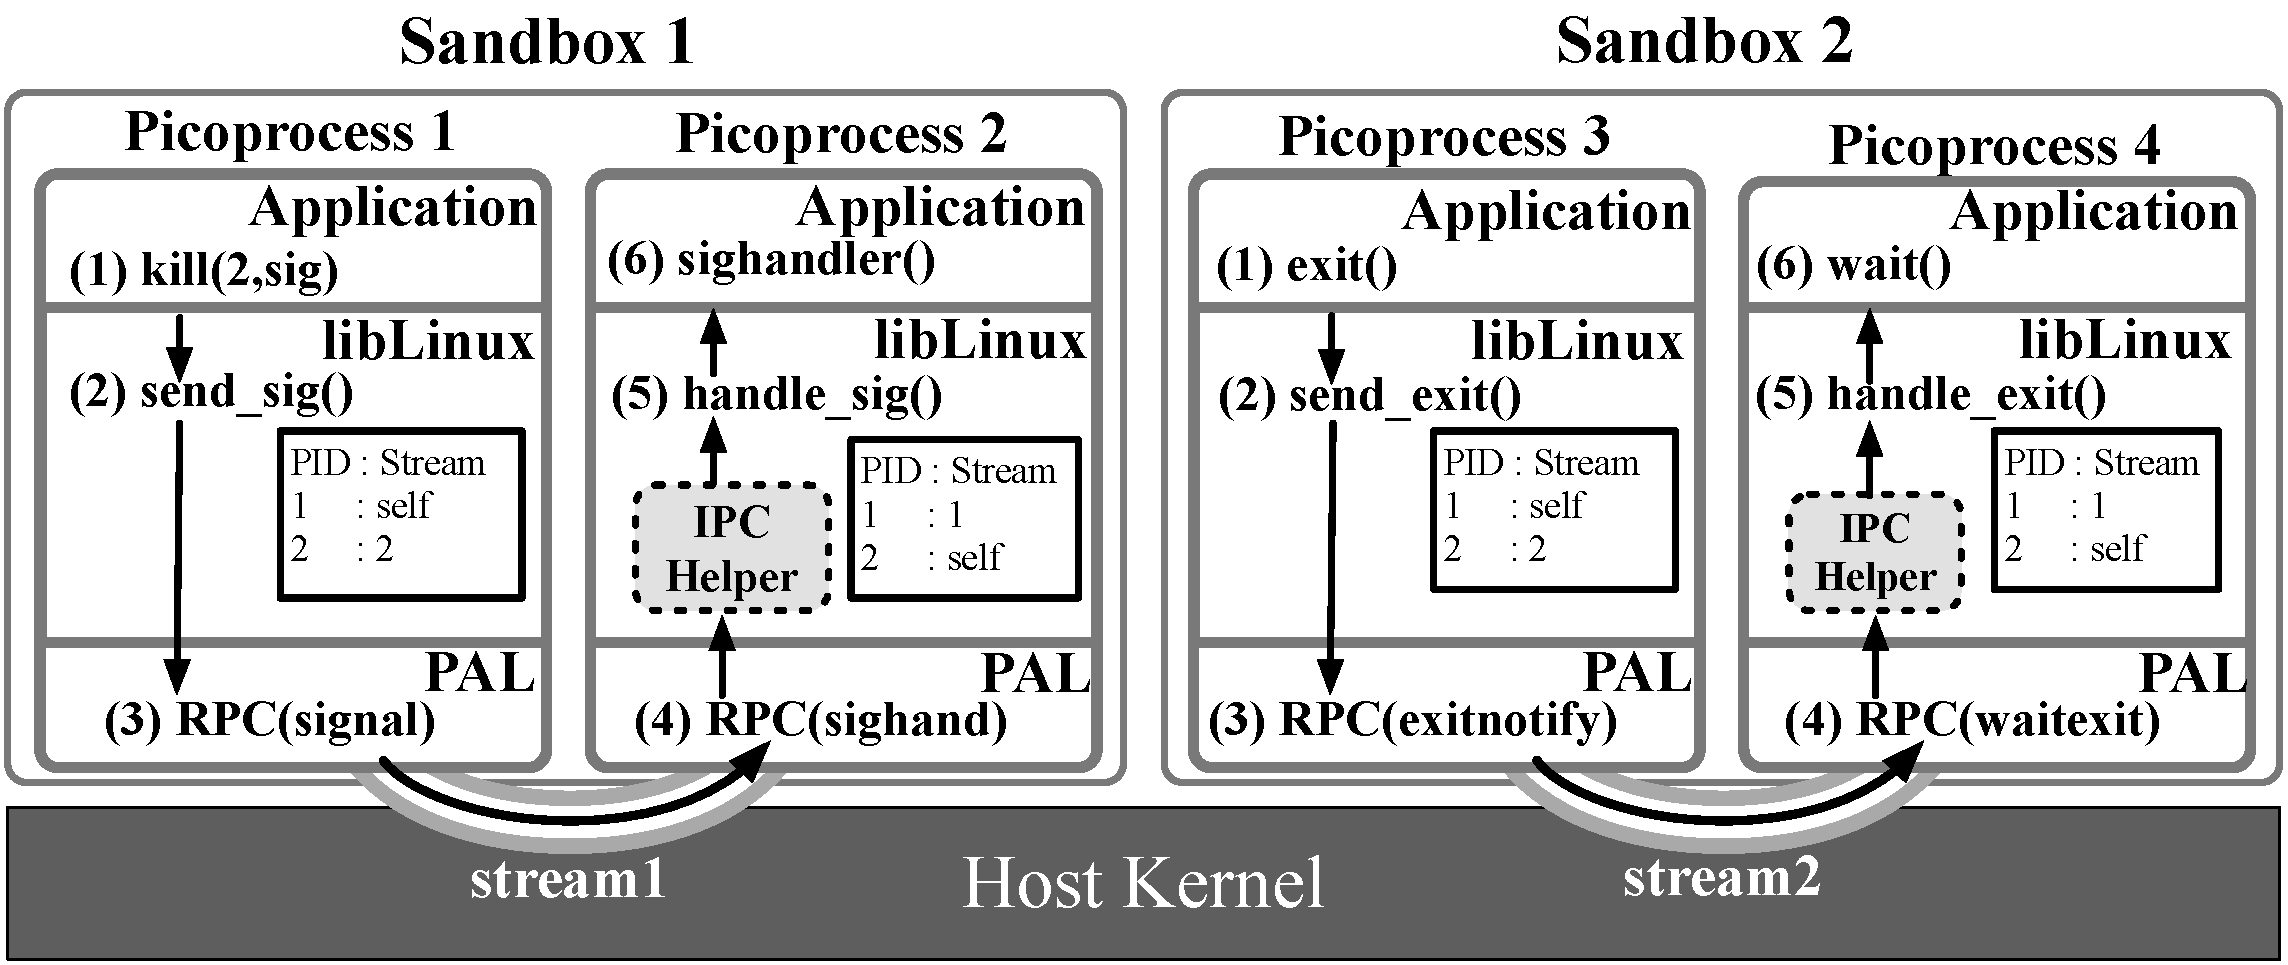
\includegraphics[width=\linewidth]{graphene/figures/coordination.pdf}
\caption{Two pairs of \graphene{} \picoprocs{} in different sandboxes 
coordinate signaling and process ID management.
The location of each PID is tracked in {\tt libLinux}; Picoprocess 1 signals
\picoproc{} 2 by sending a signal RPC over stream 1,
and the signal is ultimately delivered using a 
library implementation of the {\tt sigaction} interface. Picoprocess 4 
waits on an {\tt exitnotify} RPC from  \picoproc{} 3 over stream 2. }
\label{fig:graphene:coordination}
\end{figure}

Figure~\ref{fig:graphene:coordination} illustrates two sandboxes with \picoprocs{}
collaborating to implement a process ID (PID) namespace.  
Because PIDs and signals are a \libos{} abstraction,
\picoprocs{} in 
each sandbox can have overlapping PIDs, and
cannot signal each other.
Picoprocesses in different sandboxes cannot 
exchange RPC messages or otherwise communicate.
%If the connection between \picoprocs{} 1 and 2 is severed by subdividing the sandbox,
%the processes will become inaccessible to each other
%and each newly isolated library OS will treat the event as a process termination.


If \picoproc{} 1 (PID 1) sends a {\tt SIGUSR1} to \picoproc{} 2 (PID 2), illustrated in Figure~\ref{fig:graphene:coordination},
the {\tt kill} call to {\tt libLinux} will check its cached mapping of PIDs to 
point-to-point streams.
If {\tt libLinux} cannot find a mapping, it may begin by sending a query to the leader
to find the owner of PID 2,
and then establish a coordination stream to \picoproc{} 2.
%The leader may also pass a point-to-point coordination stream handle.
Once this stream is established, \picoproc{} 1 can send a  
signal RPC to \picoproc{} 2 (PID 2).
When \picoproc{} 2 receives this RPC, 
{\tt libLinux} will then query its local {\tt sigaction} 
structure and mark {\tt SIGUSR1} as pending.
The next time \picoproc{} 2 makes a {\tt libLinux} call,
the {\tt SIGUSR1} handler will be called upon return. Also in Figure~\ref{fig:graphene:coordination}, \picoproc{} 4 (PID 2) waits on 
\picoproc{} 3 termination (in the same sandbox with PID 1). When \picoproc{} 3 terminates, it invokes the library implementation of exit, which issues
an {\tt exitnotify} RPC to \picoproc{} 4.
%In this example, \picoprocs{} in different sandboxes have the same PID number, but this does not cause conflict as they are isolated and can only communicate with processes in the same sandbox.

%%% Using a helper thread alongside each process to asynchro-
%%% nously handle signaling
%%% is common in many \microkernel{}-based OSes such as GNU Hurd~\cite{hurd}.
%%% GNU Hurd also maintains local mappings of PIDs and RPC ports for inter-process messaging.
%%% However, PID namespace in GNU Hurd is only tracked between the parents/children, so signaling cannot be transferred between arbitrary processes.
%%% \graphene{} handles PID namespace with global consistency inside a sandbox,
%%% but requires no intensive RPCs to any centralized service.   

The \graphene{} {\tt libLinux} signal semantics closely match Linux behavior, which
delivers signals upon return from a system call or an interrupt or trap handler (\pal{} upcall).
%Each process and thread have {\tt sigaction} structures adapted from the Linux source 
%that implement the
%POSIX specification, including handler functions, as well as masking signals and
%reentrant behavior.
The {\tt libc} signal handling code is unmodified on \graphene{}.
%We extend the \pal{} with ABIs for explicit upcalls on certain hardware exceptions, such
%as divide-by-zero or segmentation faults.
%Signals from other processes, such as {\tt SIGUSR1}, are generally delivered upon 
%return from a call into {\tt libLinux}; 
If an application has a signal pending for too long,
e.g., the application is in a CPU-intensive loop, {\tt libLinux} can use a \pal{} function to interrupt 
the thread. 


% Daniela Oliveira commented. old caption for coordination
%\caption{\graphene{} namespace coordination example.  
 % Two applications and {\tt libLinux} instances
 % coordinate signaling and process ID management.
 % The location of each PID is tracked in {\tt libLinux};
 % a signal message is sent over a host stream
 % using the {\tt action} message, 
 % and the signal is ultimately delivered using a 
 % library implementation of the {\tt sigaction} interface.
%}


\begin{comment}
\graphene{} internally indexes point-to-point handles using PIDs.
In order to facilitate reallocation of PIDs without global coordination, 
\graphene{}-internal PIDs also include a {\em generation number},
allowing \picoprocs{} to lazily detect reuse similar to generation numbers 
for inodes in NFS~\cite{sandberg85nfs}.
\end{comment}

\paragraph{System V IPC.} System V IPC
maps an application-specified key onto a unique identifier.
All System V IPC abstractions, including message queues and semaphores,
are then referenced by this identifier (ID).
Similar to PIDs, 
%In order to service IPC requests, including identifier creation, from local state,
the leader divides the ID space among the \picoprocs{}, so that any \picoproc{}
can allocate an ID from local state. %a pre-allocated range.
The leader also dynamically allocates keys to \picoprocs{}.
%%% Global coordination is required to ensure that the same key maps to the same queue ID;
%%% the leader caches this information, but the owner of the queue ID or the semaphore ID 
%%% makes the definitive decision about whether a ID mapping is still valid.
%%% A key which does not have a valid mapping can be assigned to an ID by any \picoproc{}.

\paragraph{Message Queues.} In \graphene{}, the owner of a queue ID is responsible for 
storing the messages written to the queue; all message sends and receives must 
go through the owning \picoproc{}.  
In our initial implementation, any sends to or receives from a remote queue were several
orders of magnitude slower than an access to a local queue.
This led to two essential optimizations.  
First, sending to a remote
message queue was made asynchronous.  In the common case, the sender can simply assume 
the send succeeded, as the existence and location of the queue have already been determined.
The only risk of failure arises when another process deletes the queue.
When a queue is deleted, the owner sends a deletion notification to all other \picoprocs{}
that previously accessed the queue.
If a pending message was sent concurrently with the deletion notification 
(i.e., there is an application-level race condition), 
the message is treated as if it were sent after the deletion and thus dropped.
The second optimization migrates queue ownership from the producer to the consumer,
which must read queue contents synchronously.

%\fixmedp{bill: it is referenced in the Semaphores section, but here there isn't any talk about migrating msg queues to the most active \picoproc{}. also, the section starts with ``two essential optimizations. First \ldots'', but there isn't a second. is queue ownership migration the second?}

Because non-concurrent processes can share a message queue,
our implementation also uses a common file naming scheme to serialize message queues to disk.
If a \picoproc{} which owns a message queue exits, 
any pending messages are serialized to a file,
and the receiving process may request ownership of the queue from the leader.
%In order to prevent happens-before violations in case of failure, 
%message queues may be checkpointed more aggressively.


%\paragraph{Failure Recovery.}
%\label{sec:namespaces:failurerecovery}
%The \graphene{} coordination protocols are designed such that the leader does not store any unrecoverable information---the leader
%only caches the current name allocations.
%Because we assume that \picoprocs{} within a sandbox trust each other, 
%a new leader can simply broadcast a request to 
%recreate the current name allocations.  
%If the leader crashes, a simple leader election protocol is sufficient, e.g., picking the smallest live PID.

%\daniela{I wonder if the remainder of this section should be part of implementation details(section 5)}

\paragraph{Semaphores.} IPC semaphores 
follow a similar pattern to message queues, where ownership of a given semaphore is migrated
to the \picoproc{} that most frequently acquires the semaphore.
%If the owner of a semaphore exits, \graphene{} transfers ownership to the leader.  rather than serialize the semaphore to disk.
Most of the overhead in the Apache benchmark (\S\ref{sec:graphene:eval:perf}) is attributable to semaphore overheads.
%and, in ongoing work, we will likely optimize this by 
%either expanding the host ABI to share synchronization primitives within a sandbox,
%using shared memory to reduce semaphore latency.

\paragraph{Shared File Descriptors.} 
Open handle descriptors in the \graphene{} host ABI do not include a seek pointer; 
Unix-style seek behavior is implemented in the library OS.
The default Linux behavior is that children copy the open handles and file seek cursors,
but subsequent cursor movements are not shared between parent and child.
Shared file descriptor table can be requested by passing the {\tt CLONE\_FILES} flag to the {\tt clone} system call.
Any new file descriptor opened in a shared table will be visible by every process cloned in this way, as well as subsequent cursor update.
%None of our target applications have required a shared seek cursor, and it is not currently implemented,
%but would be a straightforward extension to current RPC mechanisms.
%We expect that the current RPC mechanisms could easily be extended to synchronize a seek pointer among \picoprocs{}.
If multiple \picoprocs{} are sharing file descriptor table,
the oldest one will coordinate the mapping of each file descriptor to the child \picoproc{} who owns the seek pointer.
Every update to the seek pointer will require coordination
if the \picoproc{} isn't owning it,
and similar optimization using migration can be applied here. 

\paragraph{File System States.} 
In some cases file system states need to be shared across \picoprocs{},
but the host ABI cannot export the result of Linux-specific behaviors.
For example, Linux allows user to perform specialized operations on file system
such as opening a FIFO, binding a domain socket, creating a symbolic link,
or atomically locking a file.
Coordinating these states can be cause significant slowdown on regular file system operations, so we simply export the state in regular files on the host,
 and atomically update them by renaming.

\paragraph{Shared Memory.} The \graphene{} host ABI 
does not currently permit shared memory among \picoprocs{}.
We expect that a host ABI and existing support for coordinating System V IDs would be sufficient to implement this,
with the caveat that the host must be able to handle sandbox disconnection gracefully, perhaps converting the pages to copy-on-write.
Thus far we have avoided the use of shared memory in the {\tt libLinux} implementation, both to maximize flexibility in placement of \picoprocs{}, potentially on different physical machines,
and as a rough mechanism to keep all coordination requests explicit.
%As discussed with semaphores, shared memory may also be useful to reduce latency for RPCs among picoproceses when 
%all \picoprocs{} are on the same host.


%in \graphene{} are implemented by a simple producer-consumer model.
%%% Without blocking, the latency of an inter-process semaphore operation equals to a round-trip of RPC messages.
%%% We observed that IPC semaphores can benefit from the same optimization
%%% used by message queues,
%%% based on asynchronous sending.
%%% However, when non-concurrent processes share a semaphore, it does not worth serializing the semaphore state to disk.
%%% When the owner of a semaphore exits,
%%% the semaphore state will be migrated to the leader,
%%% if it has a non-zero counter.
%%% IPC semaphores are intensively used in Apache web servers with a multi-process model. 

 
\begin{comment}
\paragraph{Limitations.} At the time of submission,
\graphene{} does not recover from all cases where a leader \picoproc{} crashes.
Our current prototype requires the IPC helper thread in the leader to remain 
in the sandbox and respond to messages even if its process {\tt main} routine has completed,
and the evaluation data reflects this state.
\end{comment}

\paragraph{Failure and Disconnection Tolerance.}  
\graphene{} is designed to tolerate disconnection of collaborating \libos{} instances,
either because of crashes or blocked RPCs.  In general, \graphene{} makes 
these disconnections isomorphic to a reasonable application behavior,
although there may be some edge cases that cannot be made completely transparent to the application.

In the absence of crashes, placing shared state in a given \picoproc{} introduces the risk that an errant 
application will corrupt shared \libos{} state.  The \microkernel{} approach of 
moving all shared state into a separate server process is more resilient to this problem.
Anecdotally, \graphene{}'s performance optimization of migrating ownership to the process that 
most heavily uses a given shared abstraction also improves the likelihood that only the corrupted
process will be affected.  
Making \graphene{} resilient to arbitrary memory corruption of any \picoproc{} is left for future work.


\paragraph{Leader Recovery.}
\graphene{} provides a leadership recovery mechanism when a leader failure is detected.
A non-leader \picoproc{} can detect the failure of a leader by either observing the shutdown of RPC streams or timing out on waiting for responses. 
Once the \picoproc{} detects leader failure, it sends out a message on the broadcast stream to volunteer for leadership.
After a few rounds of competition, the winning \picoproc{} becomes the new leader and recover the namespace state by recollecting from every other \picoproc{} in the sandbox.

%After a \picoproc{} being elected as the leader,
%the leader state,
%including all the allocated IDs and the RPC stream addresses,
%must be recovered. 
%Recollecting the leader state from all the \picoprocs{} is possible
%but can be inefficient,
%given the new leader may not have knowledge about every \picoproc{}.
%To simplify the implementation,
%we make the leaders of a namespace periodically serialize their states to disk for later recovery.

%When a \picoproc{} is sandboxed, it will detect the failure of leader because all of its RPC streams are closed by the reference monitor.
%Once it starts the leadership recovery, it will automatically win because no other \picoproc{} is sharing the broadcast stream. The procedure can be skipped by informing the sandboxed \picoproc{} before detaching.

\subsection{Lessons Learned}
\label{sec:graphene:namespaces:insights}

The current coordination design is the product of several iterations, which began 
with a fairly simple RPC-based implementation. %, and was then refined based on profiling.
This subsection summarizes the design principles that have emerged from this process.
%We present high-level facets of the design along with the insight
%behind the decision.  The next subsections synthesize these aspects 
%with specific examples of signaling and message queues.

\paragraph{Service requests from local state whenever possible.}
Sending RPC messages over Linux pipes is expensive;
this is unsurprising, given the long history of 
work on reducing IPC overhead in microkernels~\cite{liedtke93sosp,chen93memory}.  
We expect that \graphene{} performance could be improved on a 
\microkernel{} with
a more optimized IPC substrate, such as L4~\cite{liedtke95sosp,klein09sel4,elphinstone13microkernels};
we take a complementary approach of avoiding IPC if possible.
%but this is beyond the scope of our work, and we want \graphene{} to perform well on any 
%host OS.

An example of this principle is migrating message queues to the ``consumer'' when a 
clear producer/consumer pattern is detected, or migrating semaphores to the most frequent requester.
In these situations, synchronous RPC requests can be replaced with local function calls, improving
performance substantially.  For instance, migrating ownership of message queues 
reduced overhead for message receive by a factor of $10\times$.

\paragraph{Lazy discovery and caching improve performance.}  
No library OS keeps a complete replica of all distributed state,
avoiding substantial overheads to pass messages replicating irrelevant state.
Instead, \graphene{} incurs the overhead of discovering the owner of a name
on the first use, and amortizes this cost over subsequent uses.
Part of this overhead is potentially establishing a point-to-point stream,
which can then be cached for subsequent use.
For instance, the first time a process sends a signal, the helper thread 
must figure out whether the process id exists, to which \picoproc{} it maps,
and establish a point-to-point stream to the \picoproc{}.
If they exchange a second signal, the mapping is cached and reused, amortizing this 
setup cost.  For instance, the first signal a process sends to a new processes
takes \~{}2ms, but subsequent signals take only \~{}55 \us{}.

\paragraph{Batched allocation of names minimizes leader workload.}
In order to keep the leader off of the critical path of operations like {\tt fork}, 
the leader typically allocates larger blocks of names, such as process IDs or System V queue IDs.
In the case of {\tt fork}, if a \picoproc{} creates a child, it will request a batch of 
PIDs from the leader (50 by default).  Subsequent child PID allocations will be made from the same 
batch without consulting the leader.
Collaborating processes also cache the owner of a range of PIDs, avoiding 
leader queries for adjacent queries.

%% dp: Sad to see this go, but it is sort of subsumed by the other discussion
\paragraph{The coordination within a sandbox is often pairwise.}
\graphene{} optimizes the common case of pairwise coordination,
by authorizing one side of the coordination to dictate the abstraction state,
but also allows
more than two processes to share an abstraction.
Based on this insight, 
we observe that {\em not all shared state need be replicated by all \picoprocs{}}.
Instead, we adopt a design where one \picoproc{} is authoritative for a given name (e.g., a process ID or a System V queue ID).
For instance, all possible thread IDs are divided among the collaborating \picoprocs{},
and the authoritative \picoproc{} either responds to RPC requests for this thread ID (e.g., a signal)
or indicates that the thread does not exist.
This trade does make commands like {\tt ps} slower, 
but optimizes more common patterns, such as waiting for a child to exit.

\paragraph{Make RPCs asynchronous whenever possible.} 
For operations that must write to state in another \picoproc{}, 
the \graphene{} design strives to cache enough information in the sender 
to evaluate whether the operation will succeed, thereby obviating the 
need to block on the response.  This principle is applied to lower the overheads
of sending messages to a remote queue.


%this is a mapping to a thread within a specific \picoproc{}; for a message queue key,
%the mapping might be empty if the queue does not exist, or it may point to the \picoproc{} storing the pending messages.
%% The general problem underlying each of these coordination APIs is 
%% {\bf namespace management}.  In other words, coordinating \picoprocs{} need a consistent mapping
%% of names, such as a thread ID or System V message queue ID, to the authoritative \picoproc{} for that abstraction, if one exists.


\paragraph{Summary.}
The current \graphene{} design minimizes the use of RPC,
avoiding heavy communication overheads in the common case.
This design also allows for substantial flexibility to dynamically moving processes out of
a sandbox.  Finally, applications do not need to select different 
library OSes {\em a priori} based on whether they are multi-process or single-process---\graphene{}
automatically uses optimal single-process code until otherwise required.
